\begin{frame}
\frametitle{Эксперимент: Rotated Drawer World, результаты}

\begin{columns}[t]
\begin{column}{0.48\linewidth}<1->
    \begin{figure}
        \begin{subfigure}{\linewidth}
        \centering
          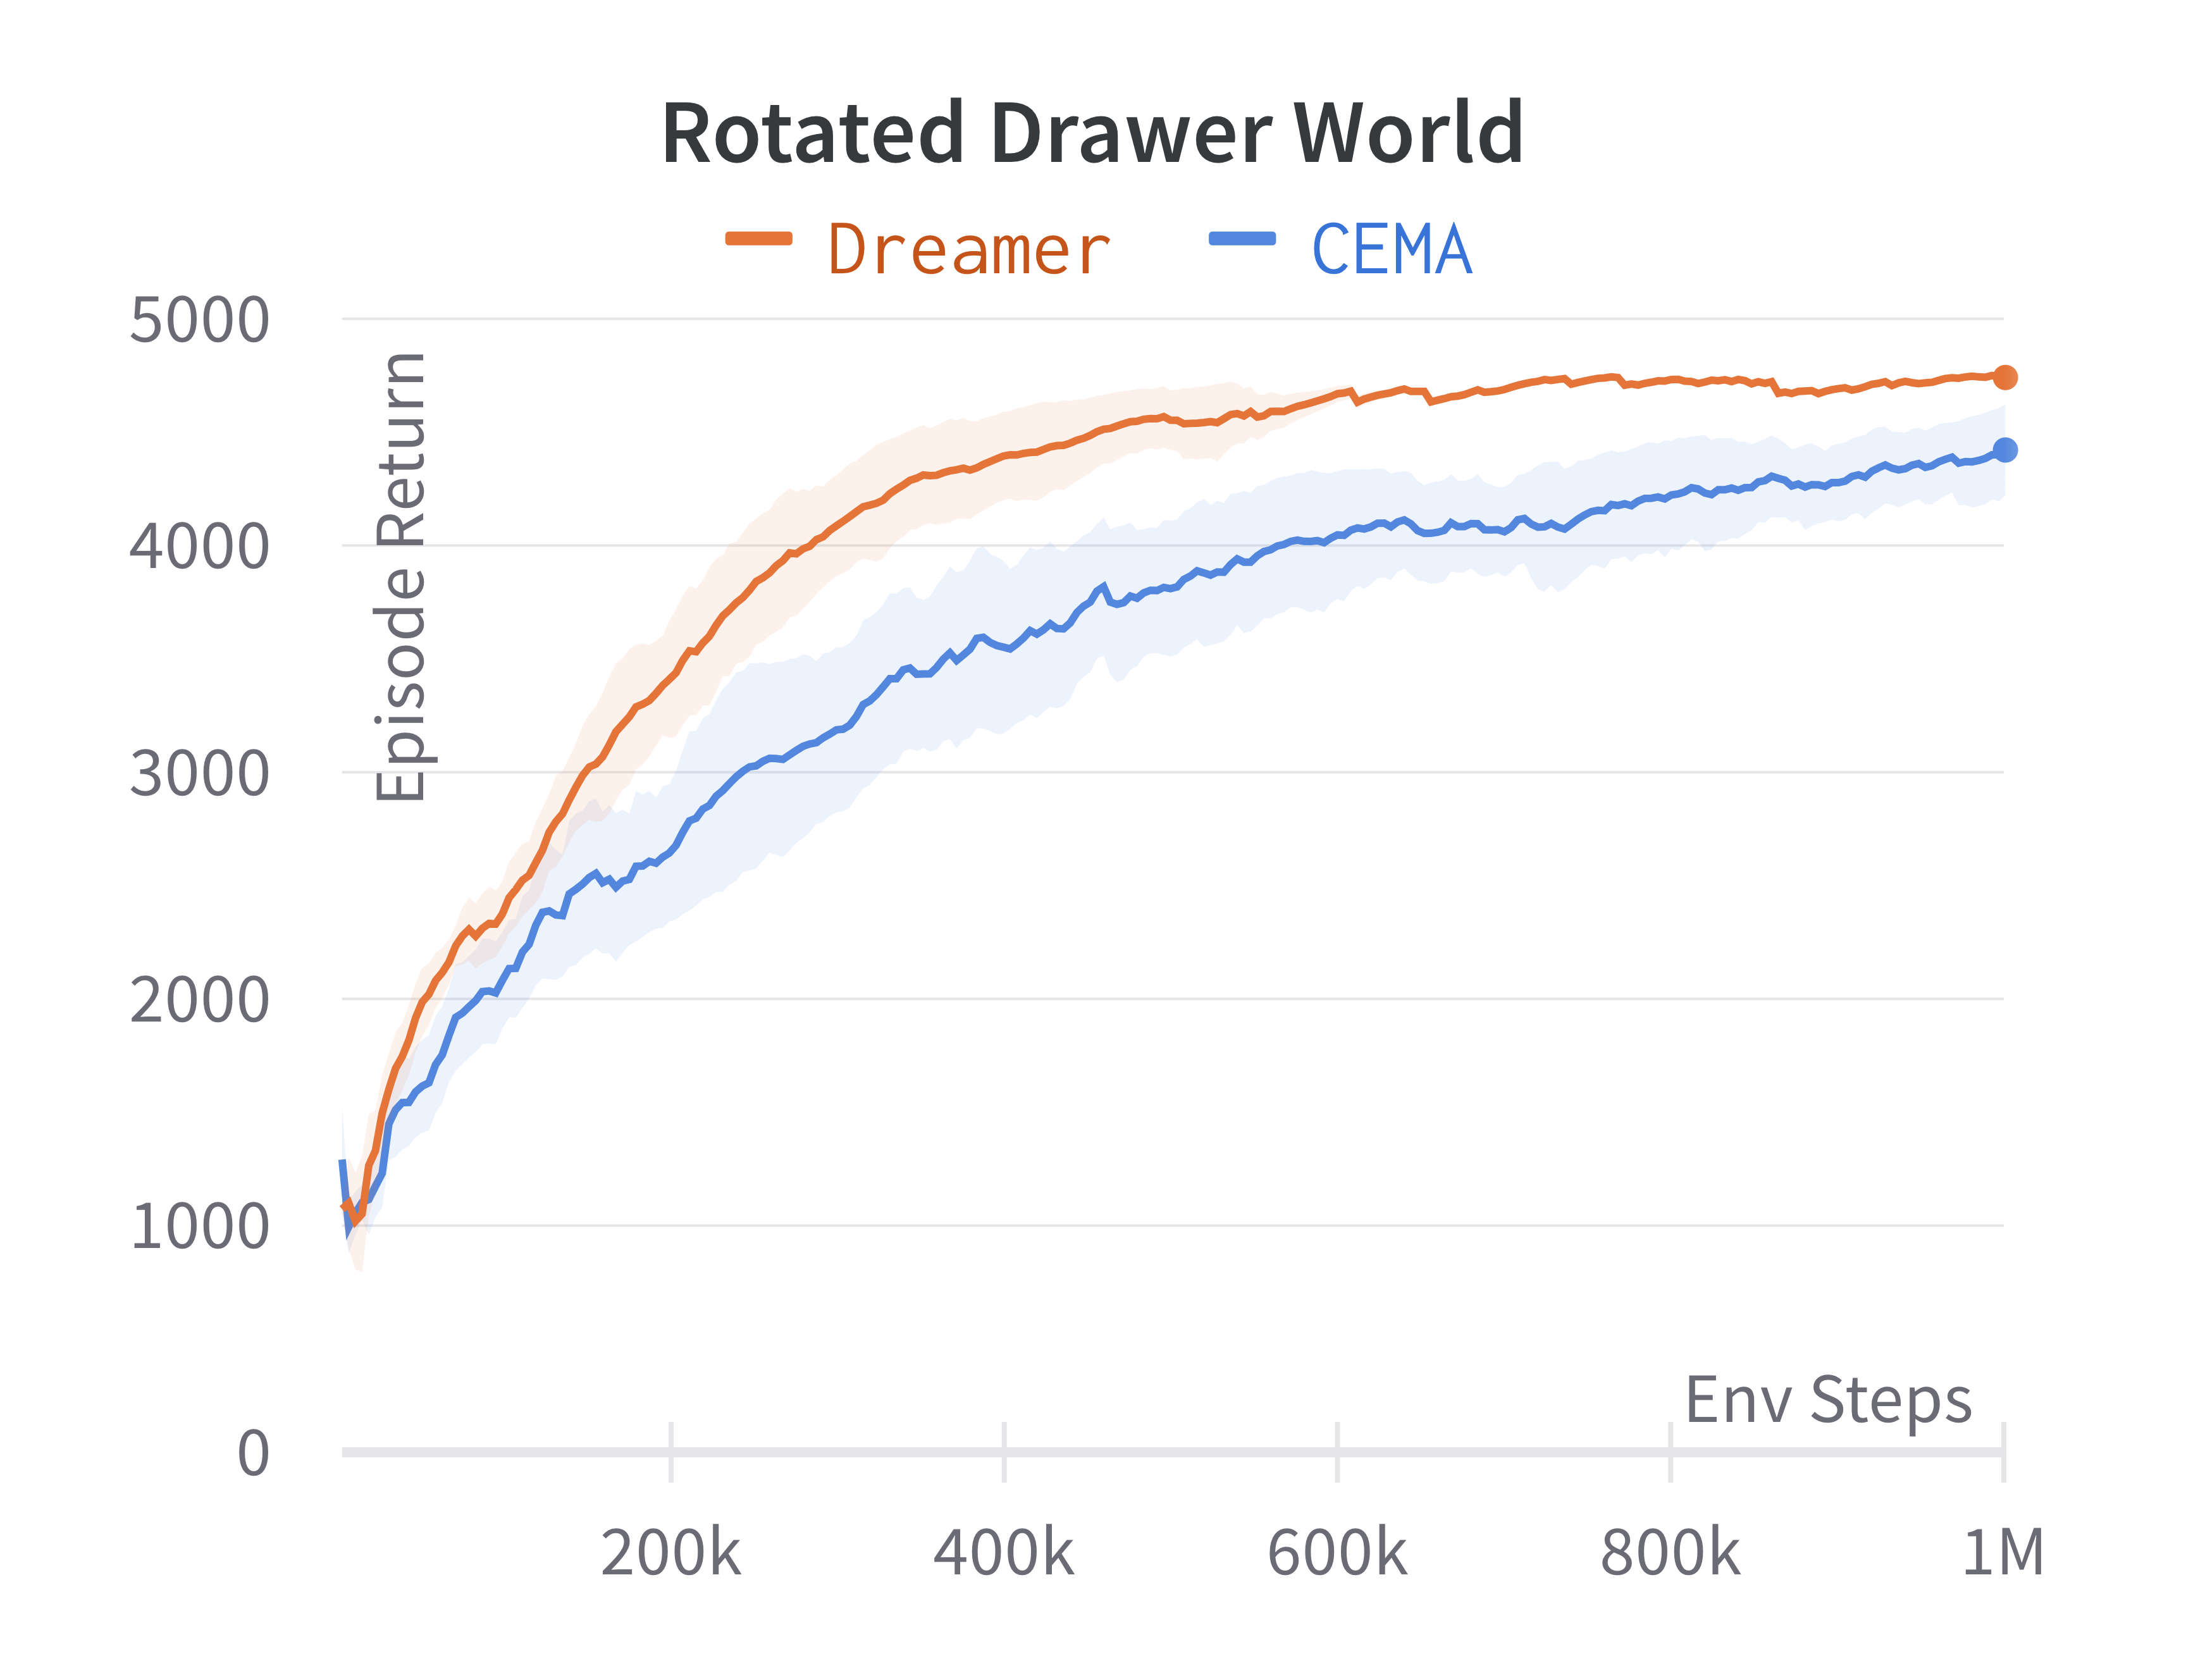
\includegraphics[height=0.5\paperheight]{images/performance/rotated_drawer_train.png}
        \end{subfigure}
      \caption{График наград на тренировочных задачах алгоритмов Dreamer и CEMA. Награды больше $3000$ соответствуют решенной задаче. }
    \end{figure}
\end{column}
\note[item]<1->{The performance of CEMA on training tasks is slightly worse than Dreamer's in terms of task solving speed.}
\hfill
\begin{column}{0.48\linewidth}<2->
    \begin{figure}
        \begin{subfigure}{\linewidth}
          \centering
          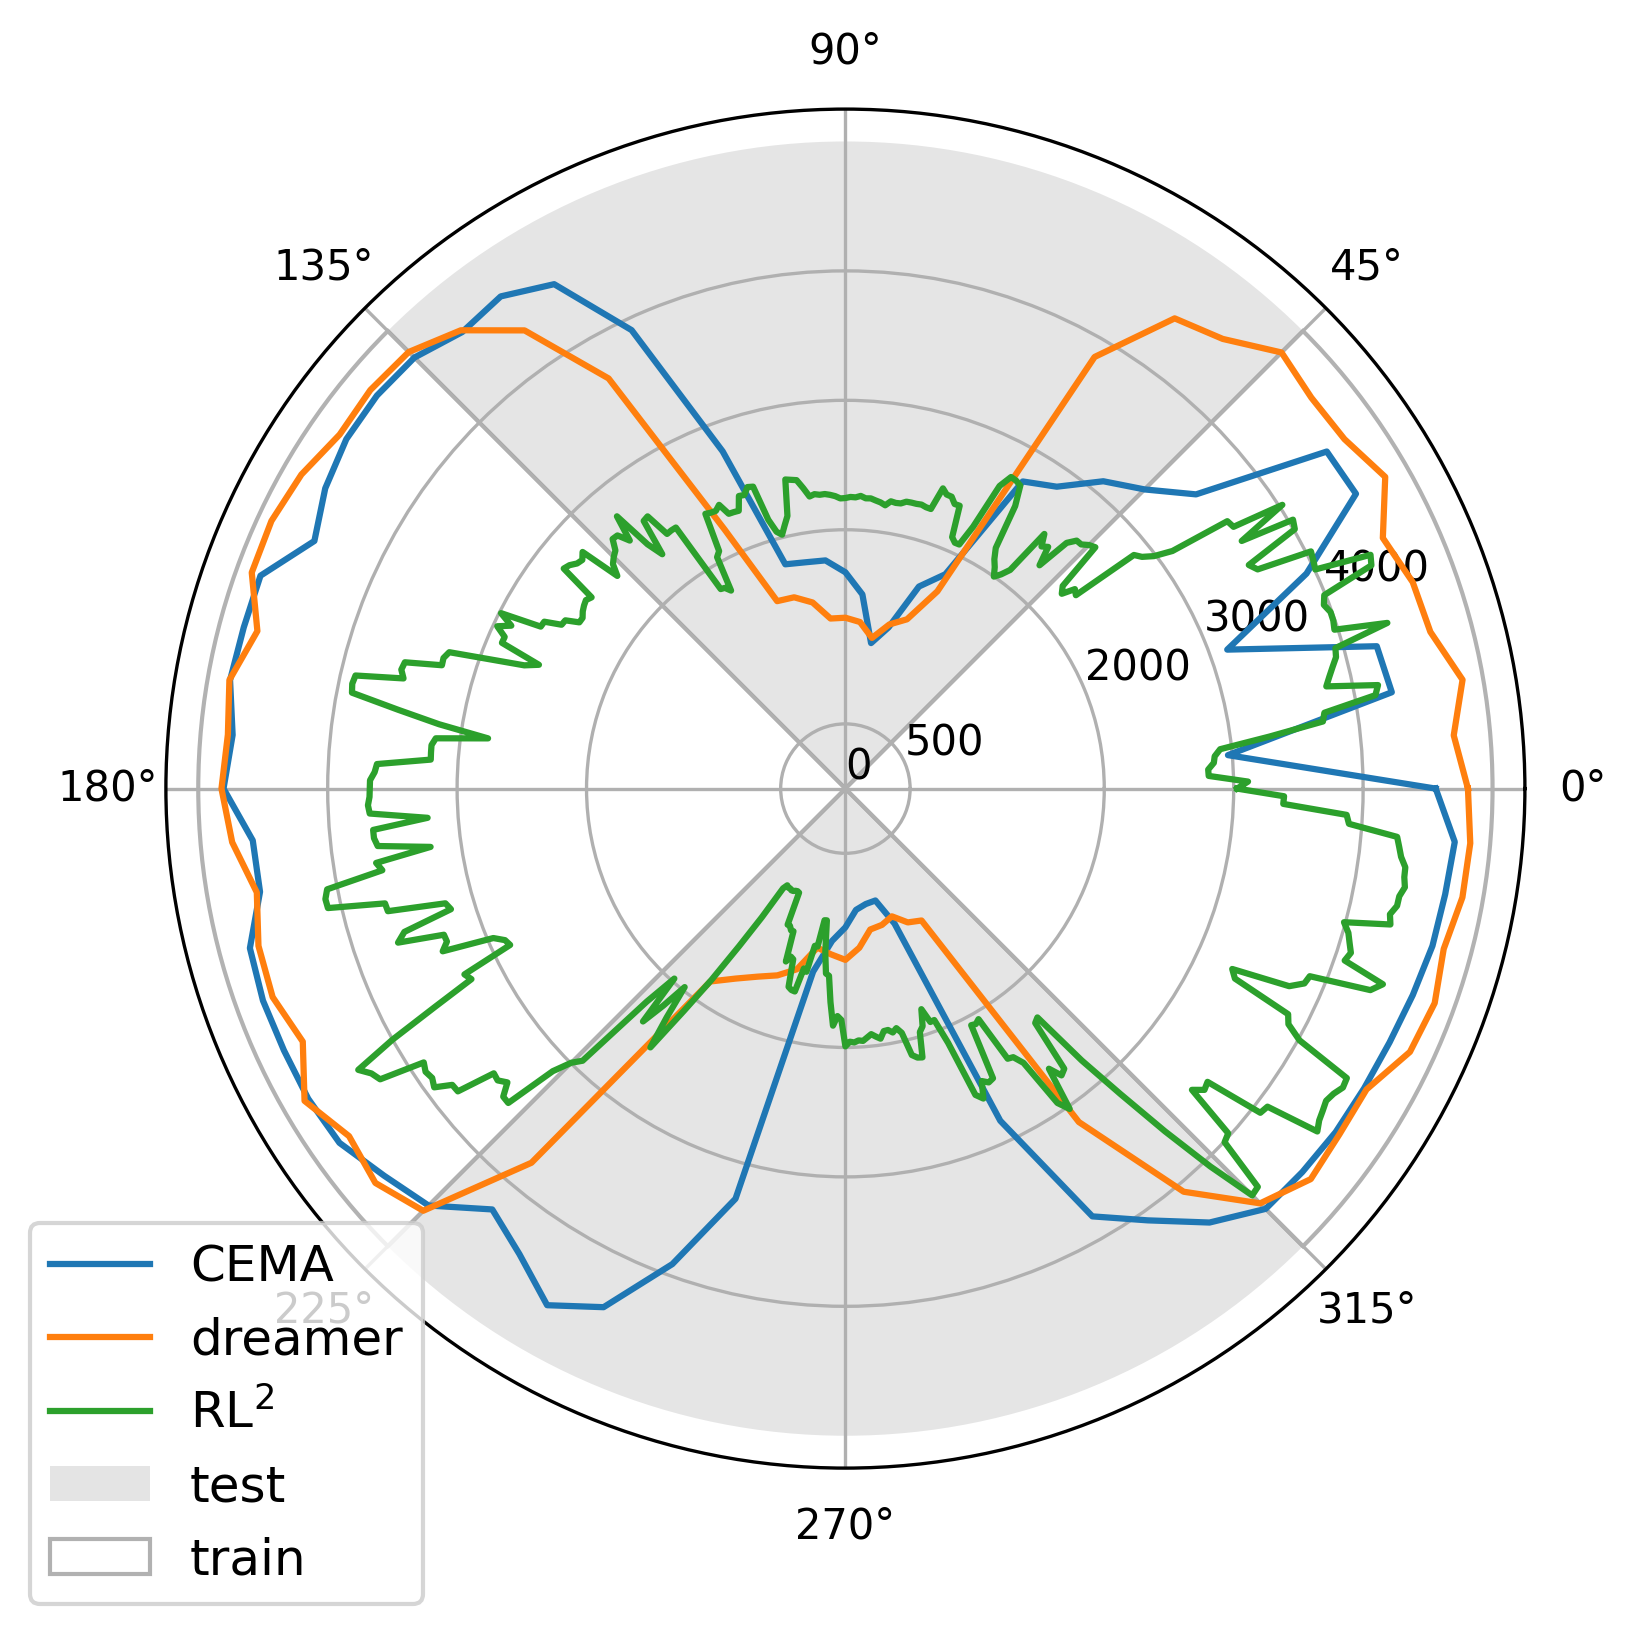
\includegraphics[height=0.5\paperheight]{images/performance/rotated_drawer_eval.png}
          \label{rd_gen_plot}
        \end{subfigure}
      \caption{Результаты работы алгоритмов на каждой задаче. Белые регионы соответствуют тренировочным задачам, синие - тестовым.}
    \end{figure}
\end{column}
\end{columns}
\note[item]<2->{However, its generalization capabilities are better - CEMA is able to solve more OOD tasks than Dreamer}
\end{frame}